%% 2020 12 25 Ph. G. Freimann @ BBW.CH
%% TALS Fct3 Polynomfunktionen

\section{Polynomfunktionen}\index{Polynomfunktionen}\index{Funktionen!Polynom-}

\subsection*{Lernziele}

\begin{itemize}
\item Polynomfunktion
\item Linearfaktoren
\item Nullstellen, Nullstellenform
\item Charakteristische Punkte
\item lokale und globale Extremwerte
\item Doppellösungen
\end{itemize}

\TALSTadBMTG{315}{18}

Rückblick über bereits bekannte Funktionen

\TNTeop{
  \begin{tabular}{|c|c|}\hline
    Polynomfunktionen   & andere Funktionen\\\hline
    $y=3$               & $\sin(x), \cos(x), \tan(x)$ \\
    $y\frac12 x -5$     & $x^{-2}, \frac{1}{x^3}$\\
    $y=2x^2-5x+3 $      & \\
    $y=(x-4)^6 + 3$     & \\\hline
    \end{tabular} 
}
%%%%%%%%%%%%%%%%%%%%%%%%%%%%%%%%%%%%%%%%%%%%%%%%%%%%%%%%%%%%%%%%%%%%%%%5

\subsection{Einstieg}
Vergleichen Sie die Graphen der Funktion
$$f: y= \frac1{10}\cdot{}(x^3-2x^2-11x+12)$$
mit demjenigen der folgenden Funktion:
$$g: y=\frac1{10}\cdot{}(x-4)\cdot{}(x+3)\cdot{}(x-1)$$


\bbwGraph{-4}{5}{-2}{3}{%%
  \TRAINER{%%
   \bbwFunc{(\x*\x*\x - 2*\x*\x - 11*\x + 12)/10}{-3.5:4.5}%% END Function
   \bbwFunc{((\x-4)*(\x+3)*(\x-1))/10}{-3.5:4.5}%% END Function
  }%% END TRAINER
}%% END bbwGraph

\newpage


\begin{beispiel}{Polynomfunktion}{}
  $$y=\LoesungsRaumLen{50mm}{4x^5 + 3x^2 -2x + 4}$$
\end{beispiel}



\begin{definition}{Polynomfunktion}{}
  Eine \textbf{Polynomfunktion} in ihrer Grundform ist eine Funktion
  der Art
  $$y = a_n\cdot{}x^n + a_{n-1}\cdot{}x^{n-1} + a_{n-2}\cdot{}x^{n-2}
  + ... + a_2\cdot{}x^2 + a_1\cdot{}x + a_0$$
  mit $a_i\in \mathbb{R}$ und $a_n\ne 0$.
\end{definition}

\begin{bemerkung}{Parabel}{}
  Parabeln sind auch Polynomfunktionen:

  $$y  = 0.3\cdot{}(2x-4)^3 + 3$$
  
\end{bemerkung}


\subsection*{Aufgaben}
%%\TALSAadBFWA{200ff}{746. $f_3$) $f_4$) $f_8$) $f_9$)}
\aufgabenFarbe{Welche der folgenden Funktionen sind Polynomfunktionen?}

$y=x^7\TRAINER{ (P)}$

$y=4x^2-0.6x^3+2x -4\TRAINER{ (P)}$

$y=x^2-\frac1{x}$

$y=(x-5)^6 + 1.5\TRAINER{ (P)}$

$y=-x^{0}\TRAINER{ (P)}$

$y=5^x-3$

$y=\frac{4x^3-2x^2-6x}{0.6}\TRAINER{ (P)}$

$y=x^{1.3}$

$y=4\TRAINER{ (P)}$

$y=\sqrt{x}$

$y=4-x^2\TRAINER{ (P)}$

$y=x^2 + x^1 + x^0 + x^{-1}$

\newpage

\subsection{gerade und ungerade Funktionen}
\subsubsection{Gerade Funktionen}

\begin{definition}{gerade Funktion}{}\index{Funktion!gerade}\index{gerade Funktion}
  Funktionen, welche an der $y$-Achse gespiegelt sind, werden
  \textbf{gerade} Funktionen genannt und haben die Eigenschaft

  $$f(x) = f(-x)$$
\end{definition}


\begin{gesetz}{gerade Exonenten}{}
  Polynomfunktionen mit ausschließlich \textbf{geraden} Exponenten sind gerade Funktionen.

  Begründung:

  $$(-x)^{2\cdot{}i} = ((-1)\cdot{}x)^{2\cdot{}i} = (-1)^{2\cdot{}i} \cdot{} x^{2\cdot{}i} = \left((-1)^2\right)^i \cdot{} x^{2\cdot{}i} = 1^i\cdot{}x^{2\cdot{}i} = x^{2\cdot{}i}$$
\end{gesetz}

\begin{beispiel}{gerade Funktion}{}
  $$g(x) = 0.3\cdot{}x^6 + 2\cdot{}x^2 + 4$$
  Bemerkung: Auch $0$ ist ein gerader Exponent:
  $$g(x) = 0.3\cdot{}x^6 + 2\cdot{}x^2 + 4\LoesungsRaum{\cdot{}x^0}$$  
\end{beispiel}
\newpage
\subsubsection{Ungerade Funktionen}
\begin{definition}{ungerade Funktion}{}\index{Funktion!ungerade}\index{ungerade Funktion}
  Funktionen, welche am Ursprung $O = (0|0)$ gespiegelt sind, werden
  \textbf{ungerade} Funktionen genannt und haben die Eigenschaft

  $$f(-x) = -f(x)$$
\end{definition}




\begin{gesetz}{\textbf{un}gerade Exponenten}{}
  Polynomfunktionen mit ausschließlich \textbf{un}geraden Exponenten sind \textbf{un}gerade Funktionen.

  Begründung:

  $$(-x)^{2\cdot{}i + 1} = ((-1)\cdot{}x)^{2\cdot{}i+1} = (-1)^{2\cdot{}i+1} \cdot{} x^{2\cdot{}i+1} = (-1)\cdot{}x^{2\cdot{}i+1} = -\left(x^{2\cdot{}i+1}\right)$$

\end{gesetz}

\begin{beispiel}{ungerade Funktion}{}
  $$g(x) = 0.3\cdot{}x^5 + 2\cdot{}x $$
  Bemerkung: Auch $x=x^1$ ist ein ungerader Exponent:
  $$g(x) = 0.3\cdot{}x^5 + 2\LoesungsRaum{\cdot{}x^1} $$  
\end{beispiel}
\newpage


\subsection*{Aufgaben}

 
\aufgabenFarbe{Zeichnen Sie Funktionen obiger beiden Beispiele mit dem
  Taschenrechner:
  $$ x \mapsto 0.3x^6+2x^2+4$$
  $$ x \mapsto 0.3x^5 + 2x$$%%
}%% End Aufgabe

\aufgabenFarbe{Trigonometrische Funktionen: Welche der Funktionen $\sin()$, $\cos()$ und $\tan()$ sind gerade, welche ungerade?}
\TNT{2.8}{
  $\sin()$ ist am Ursprung gespiegelt, somit ungerade.

  $\cos()$ ist an der $y$-Achse gespiegelt, somit gerade.

  $\tan()$ ist am Ursprung gespiegelt, somit ungerade.
}

%%\TALSAadBFWA{201}{749. a) b), 750. $f_3$) $f_4$), 751. $f_3$) $f_9$)}
\TALSAadBMTA{318}{3. und 4.}

%\aufgabenFarbe{Strukturaufgaben Seite 6 Teil 1 ohne Taschenrechner
%  Aufgabe 7. (Grad ist $n = 4$)}


\newpage

\subsection{Charakteristische Punkte und Extremwerte}

Gegeben ist der Graph der Funktion

$$f(x)=\frac1{10}(x-4)\cdot{}(x+3)\cdot{}(x-1):$$

\bbwGraph{-4}{5}{-2}{3}{%%
   \bbwFunc{((\x-4)*(\x+3)*(\x-1))/10}{-3.5:4.5}%% END Function
}%% END bbwGraph


Skizzieren Sie die im folgenden geforderten Werte und geben Sie diese
ungefähr an:

%%\renewcommand{\arraystretch}{1.5}
\begin{bbwFillInTabular}{|c|c|}\hline
  Nullstellen                   & \LoesungsRaumLang{-3, 1 und 4}\\\hline
  Extrem\textbf{stellen}        & \LoesungsRaum{$\approx -1.36$} und \LoesungsRaum{$\approx{} 2.69$}\\\hline
  Extrem\textbf{werte}          & \LoesungsRaum{$\approx 2.07 $} und \LoesungsRaum{$\approx{} -1.26$}\\\hline
  \LoesungsRaumLang{Wendepunkt} &
  $\left(\frac23\middle|\frac{11}{27}\right) = (0.\overline{6}|0.\overline{407})$\\\hline
  $y$-Achsenabschnitt           & $\left(\LoesungsRaum{0}\middle|\LoesungsRaum{1.2}\vphantom{\frac65}\right) $ \\\hline
\end{bbwFillInTabular}%%
\newpage

\subsection{Punkte-Aufgaben}

\subsection*{Einführungsaufgabe}

Gesucht ist die Polynomfunktion minimalen Grades, deren Graph durch die folgenden vorgegebenen Punkte geht:

$$(2|0); (1|-16); (0|-30); (-1|-36)$$

\TNTeop{
  1. Grad bestimmen: 4 Punkte -> 3. Grad

  2. Ansatz mit TR:
  $$f(x) := a\cdot{}x^3 + b\cdot{}x^2 + c\cdot{}x + d$$

  3. Gleichungssystem:
$$
\text{gls} := 
\left\{
\begin{array}{lcl}
f(2) &=& 0\\
f( 1) &=& -16 \\
f( 0) &=& -30\\
f(-1) &=& -36\\
\end{array}
\right.
$$

4. mit dem Solver Lösen: \texttt{solve(gls, \{a, b, c, d\})}

Lösung: $f(x) = -x^3 + 4x^2 + 11x - 30$
}%% end TNTeop
%%%%%%%%%%%%%%%%%%%%%%%%%%%%%%%%%%%%%%%%%%%%%%%%%%%%%%%%%%%%%5


\subsection*{Aufgaben}
\aufgabenFarbe{
  Gesucht ist $p$, eine Polynomfunktion 3. Grades. Die Funktion hat
  bei 2 ihren $y$-Achsenabschnitt. Ferner wissen wir, dass die Funktion die
  $x$-Achse bei $x=5$ schneidet. Zu guter Letzt geht die Funktion durch die Punkte
  $$P=\left(3\middle|\frac{-4}{5}\right), Q=\left(-1\middle|\frac{12}{5}\right)$$
  Geben Sie die Funktionsvorschrift in der Form
  $$x\mapsto ax^3 + bx^2 + cx + d$$
  an.
}%% END AufgabenFarbe

$$p: x\mapsto \LoesungsRaum{\frac{1}{15}}x^3 + \LoesungsRaum{\frac{-4}{15}}x^2 +\LoesungsRaum{\frac{-11}{15}}x + \LoesungsRaum{2}$$


\TALSAadBMTA{318}{7. a) b) c) }

\olatLinkTALSStrukturaufgabenSPF{Teil1 (ohne TR)}{6}{7. (Grad ist $n=4$)}

\olatLinkTALSStrukturaufgabenSPF{Teil 2 (mit TR)}{15ff}{48. und 51. (Bestimmen Sie zuerst die Nullstellen)}
%%\TALS{\aufgabenFarbe{Strukturaufgaben SPF Teil 2: Taschenrechner: S. 15ff:  Aufg. 48. und 51.}%% END Aufgabenfarbe
%%}%% END TALS


%%\newpage

\newpage


\subsection{Linearfaktoren und Nullstellenform}

Ziel: Wie lautet die Funktionsgleichung der folgenden Funktion?

\noTRAINER{  \bbwCenterGraphic{120mm}{tals/fct3/img/SechsLinearfaktoren.png}}
\TRAINER{  \bbwCenterGraphic{70mm}{tals/fct3/img/SechsLinearfaktoren.png}}

\newpage

\subsubsection{Voraussetzungen}

Zeichnen Sie die folgenden Polynomfunktionen mit \texttt{geogebra.org}
und diskutieren Sie Nullstellen und die Lage von Extremwerten:

\begin{itemize}
\item $f(x) = -x + 2 $ Nullstelle(n) bei \LoesungsRaum{$x=2$} 
\item $f(x) = (x+3)$ Nullstelle(n) bei \LoesungsRaum{$x=-3$}
\item $f(x) = (x+3)\cdot{}(2-x)$ Nullstelle(n) bei \LoesungsRaum{-3 und 2}
  
  Lokales Extremum
  \TNT{0.8}{zwischen -3 und 2.}%% end TNT
  
\item $f(x) = (x+3)\cdot{}(x+3)$ \LoesungsRaum{\textbf{doppelte }}
  Nullstelle bei \LoesungsRaum{$x=-3$}
  
\item $f(x) = (x-3)(x+3)(x-5)$ Nullstelle(n) bei \LoesungsRaum{$x=-3,
  3, 5$}
  
Lokale Minima/Maxima: 
  \TNT{2}{Hochpunkt zwischen -3 und 3 und Tiefpunkt zwischen 3 und 5.}
  
\item $f(x) = (-x+5)(x+3)(x+3)(x+7)$ Nullstelle(n) bei
  \LoesungsRaum{$x=-7, -3 \text{ (doppelt) und } 5$}
  
  Lokale Maxima, Minima

  \TNT{3.2}{zwischen -7 und -3; bei -3 und auch zwischen -3 und 5.}

\item $f(x) = 0.1 \cdot{} (x+1)\cdot{}(x-2)^3$\\
  Lokales Minimum zwischen \LoesungsRaumLen{30mm}{-1 und 2}.

  Die Nullstelle bei 2 wird \LoesungsRaumLen{50mm}{dreifache} Nullstelle genannt.
  
\end{itemize}


\begin{definition}{Linearfaktor}{}
  Ein Term der Form
  $$T(x) = (x+a)$$
  heißt Linearfaktor in $x$.
\end{definition}

\begin{beispiel}{Linearfaktor}{}
  Die folgende Funktion $f$ ist ein Polynom 4. Grades und hat einen
  Funktionsterm bestehend aus dem «Formfaktor» 7 sowie vier \textbf{Linearfaktoren}:
  $$f(x) = 7\cdot{}(x+3)\cdot{}(x+4)\cdot{}(x-2)\cdot{}(x+0)$$
\end{beispiel}




\newpage
\subsubsection{Grobverlauf}
Bei Polynomfunktionen reicht es, auf den Summanden mit dem höchsten Exponenten zu schauen, um den Grobverlauf des Graphen voraussagen zu können ($a$ sei $> 0$):

\noTRAINER{%%
\begin{tabular}{|c|c|}\hline
  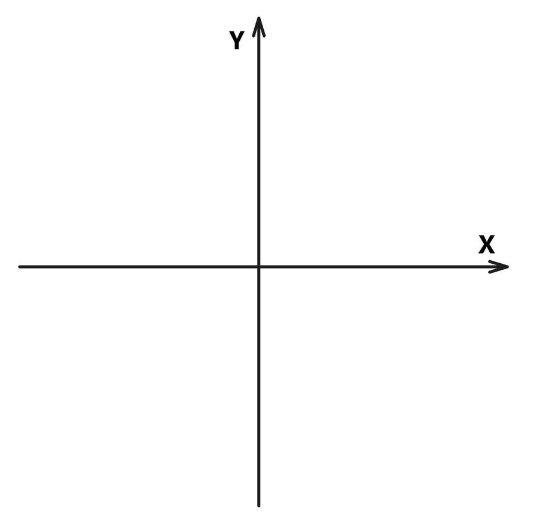
\includegraphics[width=7cm]{tals/fct3/img/KSLeer.png} &   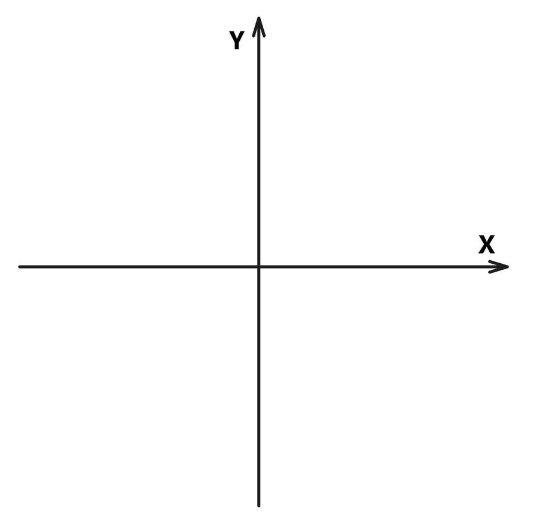
\includegraphics[width=7cm]{tals/fct3/img/KSLeer.png}\\
  $ax^4+bx^3+...$ & $-ax^4 + bx^3 +...$ \\ \hline

     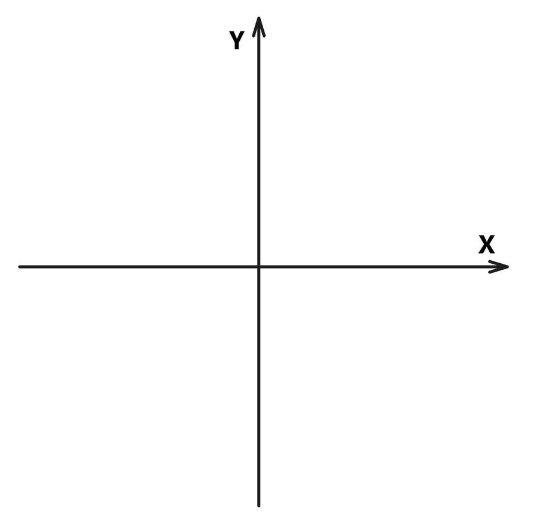
\includegraphics[width=7cm]{tals/fct3/img/KSLeer.png} &   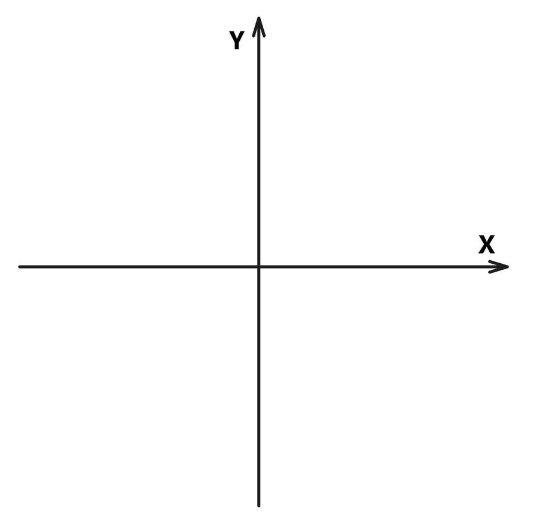
\includegraphics[width=7cm]{tals/fct3/img/KSLeer.png}\\
  $ax^5+bx^4+...$ & $-ax^5 + bx^4 +...$ \\ \hline
\end{tabular}
}%% end noTRAINER

\TRAINER{   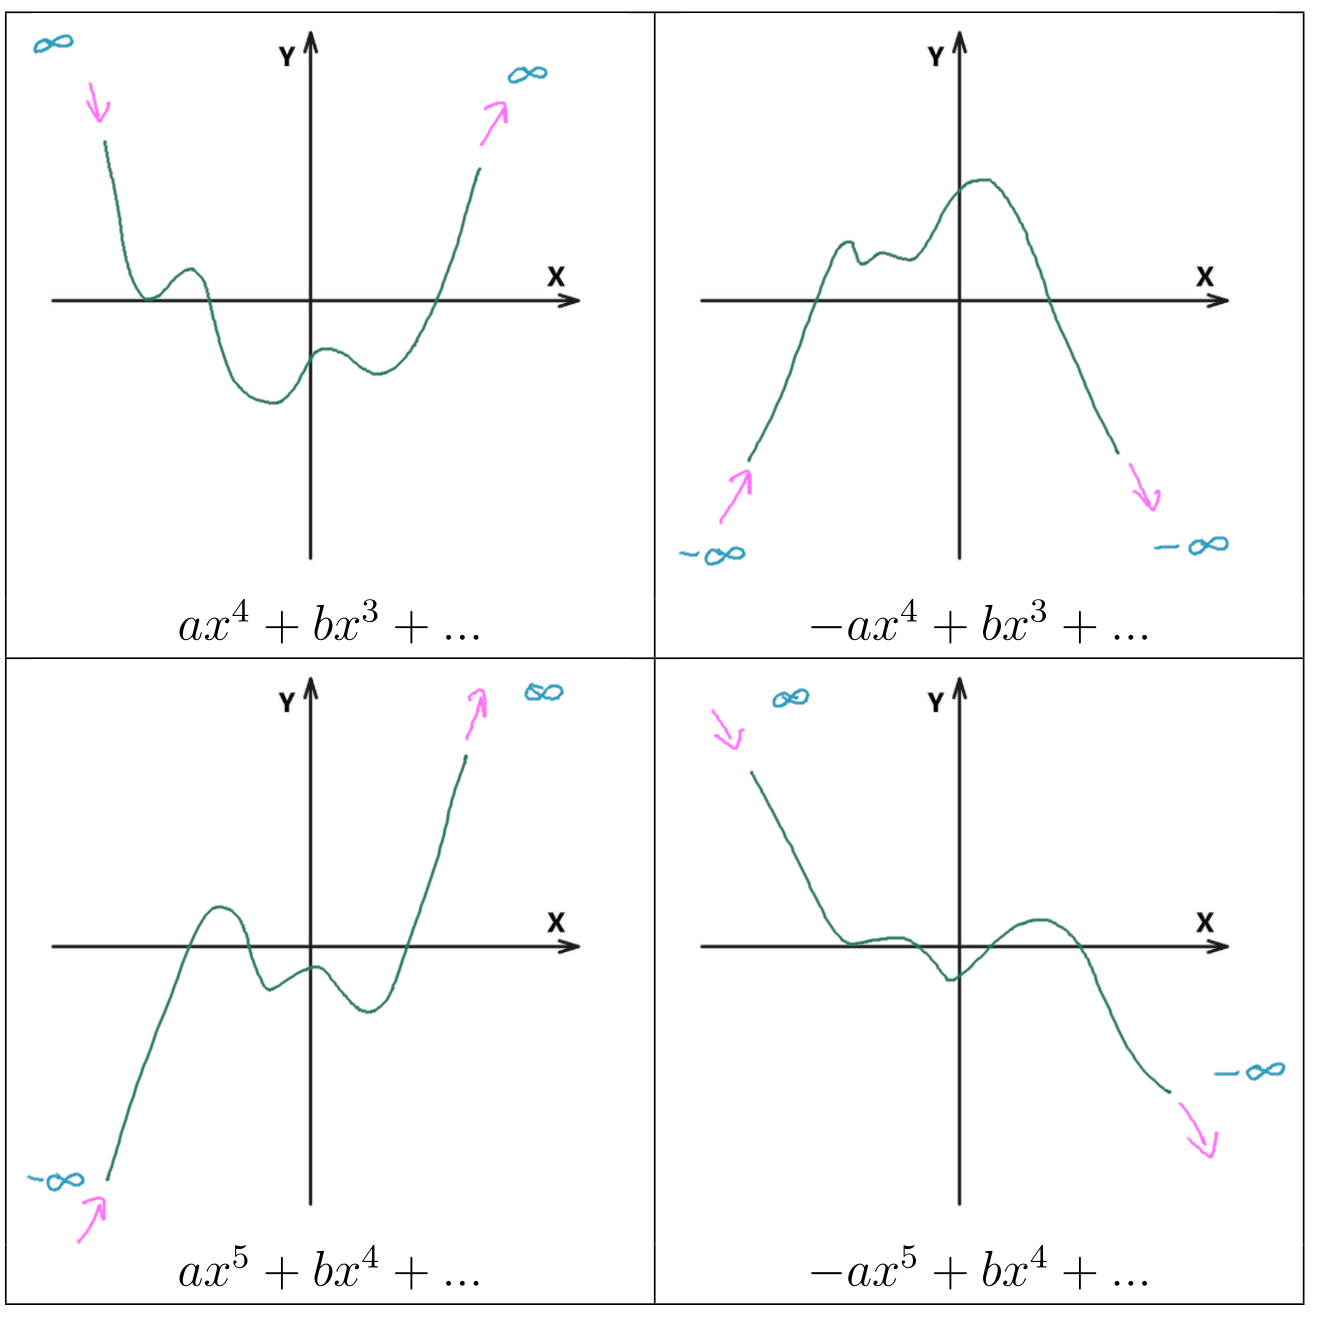
\includegraphics[width=15cm]{tals/fct3/img/Grobverlauf.png}}

\begin{rezept}{Grobverlauf}{}
  Beachten Sie nur den größten Exponenten und den zugehörigen Koeffizienten (hier $a$).

  Gerade Exponenten verhalten sich im Großen wie $x^2$ und ungerade wie $x^3$.

  Das Vorzeichen des Koeffizienten $a$ kann den Graphen an der $x$-Achse spiegeln.
\end{rezept}

\newpage


\subsection*{Referenzaufgabe}

\olatLinkTALSStrukturaufgabenSPF{Teil 2 [mit Taschenrechner]}{16}{52.}
%%\aufgabenFarbe{\textit{Strukturaufgabe [SPF] S. 16 Aufg 52. \textbf{mit} Taschenrechner!}
%%\\

\aufgabenFarbe{
  Die Punkte $P$, $Q$ und $R$ liegen auf dem Graphen einer Polynomfunktion 5. Grades. Ferner ist
bekannt, dass der Graph die $x$-Achse in $x = 3$ berührt und die
$y$-Achse in $(0|-144)$ schneidet.
$$ P=(5| -162)\,\,\,\,\,  Q=(-2| -176)\,\,\,\,\, R=(8| -1296)$$
a) Berechnen Sie die Funktionsgleichung.
\\
b) Skizzieren Sie den Graphen der Funktion in einer qualitativen Skizze, in der folgendes
dargestellt ist:
\begin{itemize}
\item alle Schnittpunkte mit der $x$-Achse
\item alle Hoch- und Tiefpunkte
\item der Globalverlauf der Funktion
\end{itemize} 
}%% END \aufgabenFarbe

\TNTeop{Welche Information fehlt noch? ``berührt'' ist nicht gleich
  ``schneidet''!

  Ansatz:
  $$f(x)=a(x-3)(x-3)(x-b)(x-c)(x-d)$$
  Danach ein Gleichungssystem erstellen

  Lösung:

  $$b=-4, c=-10, d=20, a=.....$$
  (und alle Vertauschungen)
}%% END TNT eop

\newpage

%%\noTRAINER{\newpage}

\subsubsection{Linearfaktoren erkennen}

\begin{rezept}{Linearfaktoren finden}{}
Gegeben ist folgender Graph:
\noTRAINER{  \bbwCenterGraphic{85mm}{tals/fct3/img/SechsLinearfaktoren.png}}
\TRAINER{  \bbwCenterGraphic{70mm}{tals/fct3/img/SechsLinearfaktoren.png}}

  mit der Eigenschaft $f(0) = -2.7$ bzw. «$f$ geht durch $P=(0|-2.7)$».
    
    \begin{enumerate}
  \item Grad bestimmen. Anzahl Nullstellen
    \TRAINER{(inkl. doppelte, dreifache)} \LoesungsRaum{6}
  \item Klammeransatz $f(x) =
    \LoesungsRaumLang{(x-\Box)(x-\Box)(x-\Box)(x-\Box)(x-\Box)(x-\Box)}$
  \item Nullstellen (inkl. doppelte\footnote{Doppelte Nullstellen heißen auch
      Nullstellen mit Vielfachheit\index{Vielfachheit} zwei (analog
      dreifach etc.).} eintragen)
    $$f(x) = \LoesungsRaumLang{(x+1)(x-1)(x-1)(x-3)(x-3)(x-3)}$$
  \item Allenfalls Vorfaktor $a$ bestimmen:
    $$f(0) = \LoesungsRaumLang{-2.7 = a \cdot{}(1)(-1)(-1)(-3)(-3)(-3)}$$
    $$\Longrightarrow a= \LoesungsRaumLang{\frac{-2.7}{(-3)(-3)(-3)}}$$
    $$a  = \LoesungsRaumLang{\frac{-2.7}{-27} = 0.1}$$

  \item Lösung: $f() = \LoesungsRaumLang{0.1 (x+1)(x-1)^2(x-3)^3}$ 
    \end{enumerate}
  
  \end{rezept}
\newpage


\subsection*{Aufgaben}

\aufgabenFarbe{Gesucht ist eine Polynomfunktion $f$ mit den Nullstellen $-3$, $6$ und $8$, welche durch den Punkt $(4|3)$ verläuft.}

\TNT{4}{
  Ansatz: $f(x) = a\cdot{}(x+3)(x-6)(x-8)$

  Punkt $(4|3)$ einsetzen:

  $$3 = a\cdot{}(4+3)(4-6)(4-8) = a\cdot{}56$$
  ergo: $a=\frac{3}{56}$ und somit
  $$f(x) = \frac{3}{56}(x+3)(x-6)(x-8)$$
}


\aufgabenFarbe{Gesucht ist eine Polynomfunktion $g$, welche die $x$-Achse in $x_0=7$ berührt und durch den Punkt $(1|6)$ verläuft.}

\TNT{6}{
  Ansatz: $f(x) = a\cdot{}(x-7)(x-7)$

  Punkt $(1|6)$ einsetzen:

  $$6 = a\cdot{}(1-7)(1-7) = 36 a$$
  ergo: $a=\frac{1}{6}$ und somit
  $$f(x) = \frac{1}{6}(x-7)(x-7)$$
}



\olatLinkTALSStrukturaufgabenSPF{Teil 1 [ohne TR]}{6}{6. und 10.}
%%\aufgabenFarbe{Strukturaufgaben: SPF V. 4.0 Seite 6ff: \textbf{Ohne} Taschenrechner: Aufg. 6. und 10.}

\TNTeop{}%%\noTRAINER{\mmPapier{10}}

\newpage


%%%%%%%%%%%%%%%%%%%%%%%%%%%%%%%%%%%%%%%%%%%%%%%%%%%%%%%%%%%%%%%%
\subsection{Extremwertaufgaben}

\AadBMTA{321}{17.}


\subsubsection{Aus alter Maturprüfung}

\aufgabenFarbe{Gegeben ist die Funktion $f(x) = x\cdot{}(3-\sqrt{x})$,
  $x\in[0;\infty[$.\\
  a) Bestimmen Sie die Nullstellen und das  Extremum der Funktion
  $f$.\\
  b) Im ersten Quadranten, zwischen dem  Graphen und der
  $x$-Achse ist ein  rechtwinkliges Dreieck $ABC$ einbeschrieben.  Der
  rechte Winkel ist in der Ecke $B$.  Punkt $A$ liegt im Ursprung, $B$
  auf der  $x$-Achse und $C$ auf dem Graphen von $f$. Berechnen Sie
  die Koordinaten des  Punktes $C$ so, dass der Flächeninhalt des
  Dreiecks maximal wird.
}%% END aufgabenFarbe

    
\bbwCenterGraphic{8cm}{tals/fct3/img/Maximieren.png}
\TNTeop{
   a) solve$(f(x)=0,x)$ Somit sind die Nullstellen bei 0 und 9\\
     $fmax(f(x),x)$ liefert $x=4$ ist Maximalstelle (und auch
     Maximalwert ($f(4)=4$)\\
   b) $fmax(0.5\cdot{}x\cdot{}f(x), x)$ liefert $x = 5.76$ und
   $f(5.76) = 3.456$}%% End TNTeop
%%\newpage
